\section{Experiments}
\label{sec:experiments}

\subsection{Datasets}
\noindent\textbf{\textit{Cross-Camera}}: We train on Cityscapes~\cite{cordts2016cityscapes} (2,975 imgs) and evaluate on BDD100K~\cite{yu2020bdd100k}, reporting results on the seven categories shared by both datasets, following~\cite{saito2019strong}.

\noindent\textbf{\textit{Adverse Weather}}: We train on Cityscapes~\cite{cordts2016cityscapes} and evaluate on FoggyCityscapes~\cite{sakaridis2018semantic}, using the most challenging attenuation coefficient split (0.02) to assess robustness.

\noindent\textbf{\textit{Real-to-Artistic}}: We train on VOC~\cite{everingham2010pascal} (16,551 real imgs) and evaluate on three stylized datasets~\cite{inoue2018cross}: Clipart (1K imgs, 20 categories), Comic (2K imgs, 6 categories), and Watercolor (2K imgs, 6 categories), following~\cite{li2022cross}.

\noindent\textbf{\textit{Diverse Weather Datasets}}: We train on Daytime-Sunny (19,395 imgs) and evaluate on Night-Sunny (26,158 imgs), Night-Rainy (2,494 imgs), Dusk-Rainy (3,501 imgs), and Daytime-Foggy (3,775 imgs), following~\cite{wu2022single, lee2024object}.

% \noindent\textbf{\textit{Corruption Cityscapes}}: A test-only benchmark~\cite{michaelis2019benchmarking} evaluating 15 corruption types across five severity levels. We follow the OADG~\cite{lee2024object} settings for comparison.

\noindent\textbf{\textit{Diverse Weather DroneVehicle}}:
Based on the DroneVehicle dataset~\cite{sun2022drone}, we construct one training set and three challenging testing scenarios: \textit{Clear} (8,881 imgs), \textit{Foggy} (1,040 imgs), \textit{Dark} (13,553 imgs), and \textit{Extreme-Dark} (4,965 imgs), corresponding to different levels of visibility and illumination degradation. This extension complements existing UAV detection benchmarks by introducing diverse weather conditions, 
enabling the evaluation of domain generalization under adverse environments.
Models are trained on clear conditions and evaluated on three subsets to 
assess robustness under adverse weather and low-light environments.
More details of this dataset are in the supplementary materials.

\subsection{Implementation Details}


Our experimental setup mostly follows that of Boost~\cite{ he2025boosting} and is implemented based on MMDetection~\cite{chen2019mmdetection}. For all experiments, we use Faster R-CNN~\cite{ren2016faster} as the detection framework. For generative VFMs, the detector is equipped with an FPN~\cite{lin2017feature} and a latent diffusion model~\cite{rombach2021highresolution} as the backbone feature extractor, using frozen weights from Stable Diffusion (SD) v2.1 released by StabilityAI. For discriminative VFMs, we also use Faster R-CNN with backbones initialized from the frozen pretrained weights of DINOv2-L, DINOv3-L, and SAM-Huge. To reduce the computational cost of diffusion-based features, we follow Boost~\cite{he2025boosting} and apply a knowledge distillation strategy~\cite{wang2024crosskd}, where the diffusion-based detector acts as the teacher to guide a smaller student detector. The student model is a Faster R-CNN equipped with a ResNet-101~\cite{he2016deep} backbone. All detectors are trained with SGD using a momentum of 0.9, weight decay of 0.0001, and an initial learning rate of 0.01. Detailed implementation and model structures are provided in the supplementary material.



% BDD100K: ~ref{tab:bdd100k}

% Our experimental setup mostly follows that of GDD~\cite{he2025generalized}. We implement our framework based on MMDetection~\cite{chen2019mmdetection}.
% For generative VFMs, we adopt Faster R-CNN~\cite{girshick2015fast} with an FPN~\cite{lin2017feature} as the detector, and employ a latent diffusion model~\cite{rombach2021highresolution} as the backbone to serve as a feature extractor. The diffusion backbone uses frozen weights from Stable Diffusion (SD) v2.1 released by StabilityAI. Similar to GDD, we apply a knowledge distillation strategy~\cite{wang2024crosskd}, where the diffusion-based detector serves as the teacher to guide a smaller student detector, thereby alleviating the high computational cost of diffusion feature extraction. The student model is a Faster R-CNN equipped with a ResNet-101~\cite{he2016deep} backbone.
% For discriminative VFMs, we use the frozen pretrained weights of the DINOv2-L, DINOv3-L, and SAM-Huge models.
% We train all detectors using the SGD optimizer with a momentum of 0.9, a weight decay of 0.0001, and an initial learning rate of 0.01.
% For a more detailed description of the implementation and model structure, please refer to our supplementary material.

\input{charts/BDD}
% \begin{table}[ht]
%     \centering
%     \caption{DG Results (\%) on FoggyCityscapes.}
%     \vspace{-4pt}
%     \label{tab:FoggyCityscapes}
%     \setlength{\tabcolsep}{2pt}  % 设置统一的列间距
%     \resizebox{\columnwidth}{!}{%
%     \begin{tabular}{l|cccccccc>{\columncolor{gray!20}}c}
%     \toprule
%     \textbf{Methods} & \textbf{Bus} & \textbf{Bike} & \textbf{Car} & \textbf{Motor} & \textbf{Psn.} & \textbf{Rider} & \textbf{Train} & \textbf{Truck} & \textbf{mAP} \\
%     \midrule
%     \multicolumn{10}{c}{\textit{\textbf{DG methods}}} \\
%     DIDN~\cite{didn} \textit{\scriptsize{(\textcolor{darkblue}{CVPR'21})}} & 35.7 & 33.1 & 49.3 & 24.8 & 31.8 & 38.4 & 26.5 & 27.7 & 33.4 \\
%     FACT~\cite{fact} \textit{\scriptsize{(\textcolor{darkblue}{CVPR'21})}} & 27.7 & 31.3 & 35.9 & 23.3 & 26.2 & 41.2 & 3.0 & 13.6 & 25.3 \\
%     FSDR~\cite{fsdr} \textit{\scriptsize{(\textcolor{darkblue}{CVPR'22})}} & 36.6 & 34.1 & 43.3 & 27.1 & 31.2 & 44.4 & 11.9 & 19.3 & 31.0 \\
%     MAD~\cite{mad} \textit{\scriptsize{(\textcolor{darkblue}{CVPR'23})}} & 44.0 & 40.1 & 45.0 & 30.3 & 34.2 & 47.4 & 42.4 & 25.6 & 38.6 \\
%     DDT \footnotesize{\textit{(SD-1.5)}}\normalsize~\cite{ddt} \textit{\scriptsize{(\textcolor{darkblue}{MM'24})}} & - & - & - & - & - & - & - & - & 36.1 \\
%     GDD \footnotesize{\textit{(SD-1.5)}}\normalsize~\cite{gdd}  \textit{\scriptsize{(\textcolor{darkblue}{CVPR'25})}} & \textbf{56.2} & 50.4 & 66.7 & 39.9 & 50.2 & 59.5 & 39.9 & \textbf{38.0} & 50.1 \\
%     GDD \footnotesize{\textit{(R101)}}\normalsize~\cite{gdd}  \textit{\scriptsize{(\textcolor{darkblue}{CVPR'25})}} & 53.8 & 54.2 & 67.5 & \textbf{45.6} & 52.1 & 60.8 & \textbf{53.9} & 32.4 & 52.5 \\

%     Boost\footnotesize{ (Diff. Detector, SD-1.5)} & 53.0 & 55.4 & 68.1 & 42.1 & 51.0 & 59.9 & 39.4 & 36.4 & 50.7 \\
%     \rowcolor{lightgreen}
%     Boost\footnotesize{ (Diff. Guided, R101)} & 55.3 & \textbf{62.7} & \textbf{68.2} & 45.5 & \textbf{52.9} & \textbf{62.0} & 48.4 & 37.4 & \textbf{54.1} \\
%     \midrule
%     Ours\footnotesize{ (Diff. Detector, SD-1.5)} & 53.0 & 55.4 & 68.1 & 42.1 & 51.0 & 59.9 & 39.4 & 36.4 & 50.7 \\
%     \rowcolor{lightgreen}
%     Ours\footnotesize{ (Diff. Guided, R101)} & 55.3 & \textbf{62.7} & \textbf{68.2} & 45.5 & \textbf{52.9} & \textbf{62.0} & 48.4 & 37.4 & \textbf{54.1} \\
%     \midrule
%     \midrule
%     \end{tabular}%
%     }
% \end{table}

\begin{table}[ht]
    \centering
    \caption{DG Results (\%) on FoggyCityscapes. Best values are in \textbf{boldface}.}
    \vspace{-4pt}
    \label{tab:FoggyCityscapes}
    \setlength{\tabcolsep}{2pt}  % 设置统一的列间距
    \resizebox{\columnwidth}{!}{%
    \begin{tabular}{l|cccccccc>{\columncolor{gray!20}}c}
    \toprule
    \textbf{Methods} & \textbf{Bus} & \textbf{Bike} & \textbf{Car} & \textbf{Motor} & \textbf{Psn.} & \textbf{Rider} & \textbf{Train} & \textbf{Truck} & \textbf{mAP} \\
    \midrule
    DIDN~\cite{didn} \textit{\scriptsize{(\textcolor{darkblue}{CVPR'21})}} & 35.7 & 33.1 & 49.3 & 24.8 & 31.8 & 38.4 & 26.5 & 27.7 & 33.4 \\
    FACT~\cite{fact} \textit{\scriptsize{(\textcolor{darkblue}{CVPR'21})}} & 27.7 & 31.3 & 35.9 & 23.3 & 26.2 & 41.2 & 3.0 & 13.6 & 25.3 \\
    FSDR~\cite{fsdr} \textit{\scriptsize{(\textcolor{darkblue}{CVPR'22})}} & 36.6 & 34.1 & 43.3 & 27.1 & 31.2 & 44.4 & 11.9 & 19.3 & 31.0 \\
    MAD~\cite{mad} \textit{\scriptsize{(\textcolor{darkblue}{CVPR'23})}} & 44.0 & 40.1 & 45.0 & 30.3 & 34.2 & 47.4 & 42.4 & 25.6 & 38.6 \\
    DDT \footnotesize{\textit{(Diff. Detector, SD)}}\normalsize~\cite{ddt} \textit{\scriptsize{(\textcolor{darkblue}{MM'24})}} & - & - & - & - & - & - & - & - & 36.1 \\
    GDD \footnotesize{\textit{(Diff. Detector, SD)}}\normalsize~\cite{he2025generalized}  \textit{\scriptsize{(\textcolor{darkblue}{CVPR'25})}} & 56.2 & 50.4 & 66.7 & 39.9 & 50.2 & 59.5 & 39.9 & 38.0 & 50.1 \\
   
   
    Boost\footnotesize{ \textit{(Diff. Detector, SD)}}~\cite{he2025boosting}  \textit{\scriptsize{(\textcolor{darkblue}{ICCV'25})}}& 53.0 & \textbf{55.4} & 68.1 & 42.1 & 51.0 & 59.9 & 39.4 & 36.4 & 50.7 \\
    %\rowcolor{lightgreen}
    \rowcolor{lightgreen}
    \textbf{\textit{Ours\footnotesize{ (Diff. Detector, SD)}}} & \textbf{58.8} & 52.1 & \textbf{72.0} & \textbf{44.2} & \textbf{53.7} & \textbf{61.0} & \textbf{48.1} &\textbf{38.8} & \textbf{53.6} \\
    \midrule
     GDD \footnotesize{\textit{(Diff. Guided, R101)}}\normalsize~\cite{he2025generalized}  \textit{\scriptsize{(\textcolor{darkblue}{CVPR'25})}} & 53.8 & 54.2 & 67.5 & 45.6 & 52.1 & 60.8 & 53.9 & 32.4 & 52.5 \\
    Boost\footnotesize{ \textit{(Diff. Guided, R101)}}~\cite{he2025boosting}  \textit{\scriptsize{(\textcolor{darkblue}{ICCV'25})}}& 55.3 & \textbf{62.7} & 68.2 & 45.5 & 52.9 & \textbf{62.0} & 48.4 & \textbf{37.4} & 54.1 \\
    \rowcolor{lightgreen}
    \textbf{\textit{Ours\footnotesize{ (Diff. Guided, R101)}}} & \textbf{55.7} & 57.1 & \textbf{72.9} & \textbf{46.2} & \textbf{56.5} & 61.8 & \textbf{50.1} & 37.1 & \textbf{54.7} \\
    \midrule
     SAM & 52.0 & 47.7 & 65.9 & 41.8 & 49.2 & 54.6 & 20.8 & \textbf{34.2} & 45.8 \\
    \rowcolor{lightgreen}
    \textit{\textbf{Ours \footnotesize{(SAM backbone)}}} & \textbf{56.4} & \textbf{51.5} & \textbf{68.3} & \textbf{43.1} & \textbf{52.8} & \textbf{58.3} & \textbf{36.5} & 32.3 & \textbf{49.9} \\
        \midrule
    DINOv2 & 62.1 & 45.3 & 65.5 & 44.4 & 47.6 & 55.0 & 56.3 & 46.4 & 52.8 \\
    \rowcolor{lightgreen}
    \textit{\textbf{Ours \footnotesize{(DINOv2 backbone)}}} & \textbf{69.3} & \textbf{55.1} & \textbf{70.1} & \textbf{49.8} & \textbf{54.3} & \textbf{59.4} & \textbf{58.4} & \textbf{49.1} & \textbf{58.2} \\
    \midrule
    DINOv3 & 66.9 & 55.7 & 72.6 & 48.9 & 56.1 & 62.7 & 53.1 & 45.5 & 57.7 \\
    \rowcolor{lightgreen}
    \textit{\textbf{Ours \footnotesize{(DINOv3 backbone)}}} & \textbf{72.1} & \textbf{58.6} & \textbf{73.2} & \textbf{51.7} & \textbf{58.5} & \textbf{64.6} & \textbf{65.4} & \textbf{48.6} & \textbf{61.6} \\

   
    \bottomrule
    \end{tabular}%
    }
    \vspace{-6pt}
\end{table}

% VOC
%%%%%%%%%%%%%%%%%%%%%%%%%%%%%%%%%%%%%%%%%%%%%%%%%%%%%%%%%%%%%%%%%%%%%%%%%%%%%%%%%%%%%%%%%%%%%%%%%%%%%%%%%%%%%
\begin{table}[ht]
    \centering
    \caption{DG Results (\%) on Clipart, Comic, and Watercolor. Best values are in \textbf{boldface}.}
    \vspace{-4pt}
    \label{tab:voc}
    \renewcommand{\arraystretch}{1}
    \setlength{\tabcolsep}{10pt}  % 列间距加大一点
    \resizebox{\columnwidth}{!}{%
    \begin{tabular}{l|ccc|>{\columncolor{gray!20}}c}
    \toprule
    \textbf{Methods} & \textbf{Cli.} & \textbf{Com.} & \textbf{Wat.} & \textbf{Average} \\ 
    \midrule
    Div.~\cite{Diversification} \textit{\scriptsize{(\textcolor{darkblue}{CVPR'24})}} & 33.7 & 25.5 & 52.5 & 37.2 \\
    DivAlign~\cite{Diversification} \textit{\scriptsize{(\textcolor{darkblue}{CVPR'24})}} & 38.9 & 33.2 & 57.4 & 43.2 \\
    DDT\footnotesize{ \textit{(Diff. Detector, SD)}}\normalsize~\cite{ddt} \textit{\scriptsize{(\textcolor{darkblue}{MM'24})}} & 47.4 & 44.4 & 58.7 & 50.2 \\
    GDD\footnotesize{ \textit{(Diff. Detector, SD)}}\normalsize~\cite{he2025generalized} \textit{\scriptsize{(\textcolor{darkblue}{CVPR'25})}} & 58.3 & 51.9 & 68.4 & 59.5 \\
    Boost\footnotesize{ \textit{(Diff. Detector, SD)}}\normalsize~\cite{he2025boosting} \textit{\scriptsize{(\textcolor{darkblue}{ICCV'25})}}   & \textbf{64.1} & \textbf{55.2} & 69.7 & 63.0 \\
    \rowcolor{lightgreen}
    \textit{\textbf{Ours\footnotesize{ (Diff. Detector, SD)}}} & 63.7 & 54.9 & \textbf{71.7} & \textbf{63.4} \\
    \midrule
    GDD\footnotesize{ \textit{(Diff. Guided, R101)}}\normalsize~\cite{he2025generalized} \textit{\scriptsize{(\textcolor{darkblue}{CVPR'25})}} & 40.8 & 29.7 & 54.2 & 41.6 \\
    Boost\footnotesize{ \textit{(Diff. Guided, R101)}}\normalsize~\cite{he2025boosting} \textit{\scriptsize{(\textcolor{darkblue}{ICCV'25})}}  & 40.5 & 30.0 & \textbf{56.6} & 42.4 \\
    \rowcolor{lightgreen}
    \textit{\textbf{Ours\footnotesize{ (Diff. Guided, R101)}}} & \textbf{41.3} & \textbf{32.9} & 56.1 & \textbf{43.4} \\
    \midrule

    SAM & 36.8 & \textbf{35.8} & 48.2 & 40.3 \\
    \rowcolor{lightgreen}
    \textit{\textbf{Ours\footnotesize{ (SAM backbone)}}} & \textbf{38.0} & 34.2 & \textbf{50.9} & \textbf{41.0} \\
    \midrule
    DINOv2 & 71.9 & 54.1 & 70.2 & 65.4 \\
    \rowcolor{lightgreen}
    \textit{\textbf{Ours\footnotesize{ (DINOv2 backbone)}}} & \textbf{76.5} &\textbf{58.5}  & \textbf{73.3} & \textbf{69.4} \\
    \midrule
    DINOv3 & 79.9 & 63.6 & 74.7 & 72.7 \\
    \rowcolor{lightgreen}
    \textit{\textbf{Ours\footnotesize{ (DINOv3 backbone)}}} & \textbf{81.0} & \textbf{64.1} & \textbf{74.9} & \textbf{73.3} \\
    
    \bottomrule
    \end{tabular}%
    }
\end{table}
%%%%%%%%%%%%%%%%%%%%%%%%%%%%%%%%%%%%%%%%%%%%%%%%%%%%%%%%%%%%%%%%%%%%%%%%%%%%%%%%%%%%%%%%%%%%%%%%%%%%%%%%%%%%%


% % DWD
% %%%%%%%%%%%%%%%%%%%%%%%%%%%%%%%%%%%%%%%%%%%%%%%%%%%%%%%%%%%%%%%%%%%%%%%%%%%%%%%%%%%%%%%%%%%%%%%%%%%%%%%%%%%%%
% \begin{table}[ht]
%     \centering
%     \caption{DG Results (\%) on Diverse Weather Datasets.}
%     \vspace{-4pt}
%     \label{tab:dwd}
%     \setlength{\tabcolsep}{8pt}
%     \resizebox{1\columnwidth}{!}
%     {
%     \begin{tabular}{l|cccc|>{\columncolor{gray!20}}c}
%     \toprule
%     \textbf{Methods} & \textbf{DF} & \textbf{DR} & \textbf{NR} & \textbf{NS} & \textbf{Average} \\ \midrule
%     CDSD~\cite{cdsd} \textit{\scriptsize{(\textcolor{darkblue}{CVPR'22})}} & 33.5 & 28.2 & 16.6 & 36.6 & 28.7 \\
%     SHADE~\cite{shade} \textit{\scriptsize{(\textcolor{darkblue}{ECCV'22})}} & 33.4 & 29.5 & 16.8 & 33.9 & 28.4 \\
%     CLIPGap~\cite{clip_gap} \textit{\scriptsize{(\textcolor{darkblue}{CVPR'23})}} & 32.0 & 26.0 & 12.4 & 34.4 & 26.2 \\
%     SRCD~\cite{srcd} \textit{\scriptsize{(\textcolor{darkblue}{TNNLS'24})}} & 35.9 & 28.8 & 17.0 & 36.7 & 29.6 \\
%     G-NAS~\cite{gnas} \textit{\scriptsize{(\textcolor{darkblue}{AAAI'24})}} & 36.4 & 35.1 & 17.4 & 45.0 & 33.5 \\
%     PhysAug~\cite{physaug} \textit{\scriptsize{(\textcolor{darkblue}{ArXiv'24})}} & 40.8 & 41.2 & 23.1 & 44.9 & 37.5 \\ 
%     OA-DG~\cite{lee2024object} \textit{\scriptsize{(\textcolor{darkblue}{AAAI'24})}} & 38.3 & 33.9 & 16.8 & 38.0 & 31.8 \\
%     DivAlign~\cite{Diversification} \textit{\scriptsize{(\textcolor{darkblue}{CVPR'24})}} & 37.2 & 38.1 & 24.1 & 42.5 & 35.5 \\
%     UFR~\cite{ufr} \textit{\scriptsize{(\textcolor{darkblue}{CVPR'24})}} & 39.6 & 33.2 & 19.2 & 40.8 & 33.2 \\
%     Prompt-D~\cite{prompt-d} \textit{\scriptsize{(\textcolor{darkblue}{CVPR'24})}} & 39.1 & 33.7 & 19.2 & 38.5 & 32.6 \\
%     DIDM~\cite{didm} \textit{\scriptsize{(\textcolor{darkblue}{ArXiv'25})}} & 39.3 & 35.4 & 19.2 & 42.0 & 34.0 \\
%     % GDD \footnotesize{\textit{(Diff. Detector,SD)}} \normalsize~\cite{he2025generalized}  \textit{\scriptsize{(\textcolor{darkblue}{CVPR'25})}} & 43.3 & 42.5 & 27.8 & 47.0 & 40.2 \\
%     % GDD \footnotesize{\textit{(Diff. Guided, R101)}} \normalsize~\cite{he2025generalized}  \textit{\scriptsize{(\textcolor{darkblue}{CVPR'25})}} & 44.7 & 37.4 & 21.7 & 48.7 & 38.1 \\
%     Boost^{*}\footnotesize{ \textit{(Diff. Detector,SD)}}\normalsize~\cite{he2025boosting} \textit{\scriptsize{(\textcolor{darkblue}{ICCV'25})}} &45.9 &44.3 & 28.2 &48.8 & 41.8 \\
%     Boost^{*}\footnotesize{ \textit{(Diff. Guided, R101)}}\normalsize~\cite{he2025boosting} \textit{\scriptsize{(\textcolor{darkblue}{ICCV'25})}} &44.4 & 36.1 & 20.9 & 47.7 & 37.3 \\
%     \midrule
%    % \rowcolor{lightgreen}
%     \textit{\textbf{Ours\footnotesize{ (Diff. Detector, SD)}}} & 47.5 & 47.0 & 30.2 & 51.9 & 44.2 \\
%     \textit{\textbf{Ours\footnotesize{ (Diff. Guided, R101)}}} & - & - & - & - & - \\
%     \midrule
%     DINOv2 & 40.7 & 43.8 & 33.8 & 44.7 & 40.75 \\
%     \textit{\textbf{Ours\footnotesize{ (DINOv2 backbone)}}} & 44.0 & 48.7 & 37.0 & 49.3 & 44.75 \\
%     \midrule
%     DINOv3 & 46.6 & 50.7 & 45.1 & 52.0 & 48.6 \\
%     \textit{\textbf{Ours\footnotesize{ (DINOv3 backbone)}}} & 48.1 & 53.8 & 46.7 & 54.6 & 50.8 \\
%     \midrule
%     SAM & -- & -- & -- & -- & -- \\
%     \textit{\textbf{Ours\footnotesize{ (SAM backbone)}}} & -- & -- & -- & -- & -- \\
%     \bottomrule
%     \end{tabular}
%     }
% \end{table}



\begin{table}[ht]
    \centering
    \caption{DG Results (\%) on Diverse Weather Datasets. Best values are in \textbf{boldface}. $*$Results reimplemented by us using 19,395 training images.}
    \vspace{-4pt}
    \label{tab:dwd}
    \setlength{\tabcolsep}{10pt}
    \resizebox{1\columnwidth}{!}{
    \begin{tabular}{l|cccc|>{\columncolor{gray!20}}c}
    \toprule
    \textbf{Methods} & \textbf{DF} & \textbf{DR} & \textbf{NR} & \textbf{NS} & \textbf{Average} \\ 
    \midrule
    CDSD~\cite{cdsd} \textit{\scriptsize{(\textcolor{darkblue}{CVPR'22})}} & 33.5 & 28.2 & 16.6 & 36.6 & 28.7 \\
    SHADE~\cite{shade} \textit{\scriptsize{(\textcolor{darkblue}{ECCV'22})}} & 33.4 & 29.5 & 16.8 & 33.9 & 28.4 \\
    CLIPGap~\cite{clip_gap} \textit{\scriptsize{(\textcolor{darkblue}{CVPR'23})}} & 32.0 & 26.0 & 12.4 & 34.4 & 26.2 \\
    SRCD~\cite{srcd} \textit{\scriptsize{(\textcolor{darkblue}{TNNLS'24})}} & 35.9 & 28.8 & 17.0 & 36.7 & 29.6 \\
    G-NAS~\cite{gnas} \textit{\scriptsize{(\textcolor{darkblue}{AAAI'24})}} & 36.4 & 35.1 & 17.4 & 45.0 & 33.5 \\
    PhysAug~\cite{physaug} \textit{\scriptsize{(\textcolor{darkblue}{ArXiv'24})}} & 40.8 & 41.2 & 23.1 & 44.9 & 37.5 \\ 
    OA-DG~\cite{lee2024object} \textit{\scriptsize{(\textcolor{darkblue}{AAAI'24})}} & 38.3 & 33.9 & 16.8 & 38.0 & 31.8 \\
    DivAlign~\cite{Diversification} \textit{\scriptsize{(\textcolor{darkblue}{CVPR'24})}} & 37.2 & 38.1 & 24.1 & 42.5 & 35.5 \\
    UFR~\cite{ufr} \textit{\scriptsize{(\textcolor{darkblue}{CVPR'24})}} & 39.6 & 33.2 & 19.2 & 40.8 & 33.2 \\
    Prompt-D~\cite{prompt-d} \textit{\scriptsize{(\textcolor{darkblue}{CVPR'24})}} & 39.1 & 33.7 & 19.2 & 38.5 & 32.6 \\
    DIDM~\cite{didm} \textit{\scriptsize{(\textcolor{darkblue}{ArXiv'25})}} & 39.3 & 35.4 & 19.2 & 42.0 & 34.0 \\
    Boost$^{*}$~\footnotesize{\textit{(Diff. Detector, SD)}}~\cite{he2025boosting} \textit{\scriptsize{(\textcolor{darkblue}{ICCV'25})}} &45.9 &44.3 & 28.2 &48.8 & 41.8 \\
    \rowcolor{lightgreen}
    \textit{\textbf{Ours (Diff. Detector, SD)}} & \textbf{47.5} & \textbf{47.0} & \textbf{30.2} & \textbf{51.9} & \textbf{44.2} \\
    \midrule
    Boost$^{*}$~\footnotesize{\textit{(Diff. Guided, R101)}}~\cite{he2025boosting} \textit{\scriptsize{(\textcolor{darkblue}{ICCV'25})}} &44.4 & 36.1 & 20.9 & 47.7 & 37.3 \\
    \rowcolor{lightgreen}
    \textit{\textbf{Ours (Diff. Guided, R101)}} &\textbf{44.5} & \textbf{38.4} &\textbf{22.4} & \textbf{48.6} & \textbf{38.5} \\
    \midrule
    SAM & 41.2 & 41.3 & 26.1 & 45.0 & 38.4 \\
    \rowcolor{lightgreen}
    \textit{\textbf{Ours (SAM backbone)}} & \textbf{42.7} & \textbf{44.3} & \textbf{28.6} & \textbf{48.0} & \textbf{40.9} \\
    \midrule
    DINOv2 & 40.7 & 43.8 & 33.8 & 44.7 & 40.8 \\
    \rowcolor{lightgreen}
    \textit{\textbf{Ours (DINOv2 backbone)}} & \textbf{44.0} & \textbf{48.7} & \textbf{37.0} & \textbf{49.3} & \textbf{44.8} \\
    \midrule
    DINOv3 & 46.6 & 50.7 & 45.1 & 52.0 & 48.6 \\
    \rowcolor{lightgreen}
    \textit{\textbf{Ours (DINOv3 backbone)}} & \textbf{48.1} & \textbf{53.8} & \textbf{46.7} & \textbf{54.6} & \textbf{50.8} \\
    \bottomrule
    \end{tabular}}




\end{table}

%%%%%%%%%%%%%%%%%%%%%%%%%%%%%%%%%%%%%%%%%%%%%%%%%%%%%%%%%%%%%%%%%%%%%%%%%%%%%%%%%%%%%%%%%%%%%%%%%%%%%%%%%%%%%
\begin{table}[ht]
    \centering
    \caption{DG Results (\%) on Diverse Weather (Dark, Foggy, and Extreme Dark). Best values are in \textbf{boldface}.}
    \vspace{-4pt}
    \label{tab:drone}
    \renewcommand{\arraystretch}{1}
    \setlength{\tabcolsep}{8pt}
    \resizebox{\columnwidth}{!}{%
    \begin{tabular}{l|ccc|>{\columncolor{gray!20}}c}
    \toprule
    \textbf{Methods} & \textbf{Dark} & \textbf{Foggy} & \textbf{Ext. Dark} & \textbf{Average} \\ 
    \midrule
    Faster R-CNN  & 33.1  & 54.8 &8.1 &  32.0 \\ 
     GDD \footnotesize{ \textit{(Diff. Detector, SD)}}~\cite{he2025generalized} \textit{\scriptsize{(\textcolor{darkblue}{CVPR'25})}} & {40.1} & {54.8} & {20.4} & {38.4} \\
    Boost\footnotesize{ \textit{(Diff. Detector, SD)}}~\cite{he2025boosting} \textit{\scriptsize{(\textcolor{darkblue}{ICCV'25})}} & {42.0} & \textbf{58.3} & {21.3} & {40.5} \\
    \rowcolor{lightgreen}
    \textit{\textbf{Ours\footnotesize{ (Diff. Detector, SD)}}} & \textbf{45.2} & {56.5} &  \textbf{24.2} & \textbf{42.0} \\

     \midrule
     SAM & 40.4 & 52.4  & 19.9 & 37.6 \\
     \rowcolor{lightgreen}
    \textit{\textbf{Ours\footnotesize{ (SAM backbone)}}} & \textbf{41.1} & \textbf{53.2}  & \textbf{20.7}  & \textbf{38.4} \\
    
    \midrule
    DINOv2 & 47.0 & 53.0  & 26.5 & 42.2 \\
    \rowcolor{lightgreen}
    \textit{\textbf{Ours\footnotesize{ (DINOv2 backbone)}}} & \textbf{48.9} & \textbf{58.2}  & \textbf{29.8}  & \textbf{45.6} \\
    \midrule
    DINOv3 & 50.9 &  56.7 & 33.7 & 47.1 \\
    \rowcolor{lightgreen}
    \textit{\textbf{Ours\footnotesize{ (DINOv3 backbone)}}} & \textbf{51.4} & \textbf{59.9} & \textbf{34.0}  & \textbf{48.4} \\
   
     \bottomrule
    \end{tabular}%
    }
    \vspace{-6pt}
\end{table}
%%%%%%%%%%%%%%%%%%%%%%%%%%%%%%%%%%%%%%%%%%%%%%%%%%%%%%%%%%%%%%%%%%%%%%%%%%%%%%%%%%%%%%%%%%%%%%%%%%%%%%%%%%%%%



% Our experimental setup mostly follows that of GDD~\cite{he2025generalized}. We implement our framework based on the MMDetection~\cite{chen2019mmdetection}. 
% Specifically, we adopt Faster R-CNN~\cite{girshick2015fast} with an FPN~\cite{lin2017feature} as the detector, while employing a latent diffusion model~\cite{rombach2021highresolution} as the backbone to serve as a feature extractor. 
% The diffusion backbone uses frozen weights from Stable Diffusion v2.1 released by StabilityAI.
% Similar to GDD, 
% we apply a knowledge distillation strategy, where a diffusion-based detector serves as the teacher to guide a smaller student detector, thereby alleviating the high computational cost of diffusion feature extraction.
% The student model is a Faster R-CNN equipped with a ResNet-101~\cite{he2016deep} backbone.
% We use the SGD optimizer with a momentum of 0.9 and a weight decay of 0.0001 in the initial learning rate of 0.01.

\subsection{Comparison with State-of-the-Arts}
We present quantitative results on various DG benchmarks in Tables \ref{tab:bdd100k}, \ref{tab:FoggyCityscapes}, \ref{tab:dwd}, \ref{tab:voc}, and \ref{tab:drone}, with AP$_{50}$ as the evaluation metric. 
The following abbreviations are used in the tables: 
\textbf{Com.} (Comic), \textbf{Wat.} (Watercolor), and \textbf{Cli.} (Clipart) for Table~\ref{tab:voc};
\textbf{DF} (Daytime-Foggy), \textbf{DR} (Dusk-Rainy), \textbf{NR} (Night-Rainy), and \textbf{NS} (Night-Sunny) for Table~\ref{tab:dwd};
and \textbf{Ext.~Dark} (Extreme Dark) for Table~\ref{tab:drone}.
To facilitate comparison, \textbf{\textit{Bridge}}’s performance is highlighted in \colorbox{lightgreen}{light green} in the tables.


\noindent\textbf{\textit{Cross-Camera}}:
In Table~\ref{tab:bdd100k}, we evaluate \textbf{\textit{Bridge}} on the Cross-Camera DG benchmark, where the model is trained on Cityscapes and tested on BDD100K.  
\textbf{\textit{Bridge}}, built upon a Stable Diffusion backbone (\textit{Diff.~Detector}), surpasses the previous state-of-the-art method Boost~\cite{he2025boosting} by a margin of $\mathbf{3.8}$ mAP. In addition, following the settings of Boost and GDD, we adopt the CrossKD~\cite{wang2024crosskd} technique to transfer knowledge from Stable Diffusion to a smaller backbone (\textit{Diff.~Guided, R101}), enabling lightweight deployment.  
Compared with Boost’s \textit{Diff.~Guided} detector, our model still achieves a $\mathbf{2.0}$ mAP improvement, further demonstrating that \textbf{\textit{Bridge}} can effectively exploit VFM priors for robust domain generalization, even with a compact backbone.


In terms of discriminative VFMs, \textbf{\textit{Bridge}} achieves consistent mAP improvements of $\mathbf{5.1}$, $\mathbf{1.1}$, and $\mathbf{2.0}$ over the corresponding baselines on DINOv2, DINOv3, and SAM, respectively, further demonstrating its strong generalization capability.  
Notably, we observe substantial improvements in \textit{rider}, \textit{bike}, \textit{person}, and \textit{motor}.  
These categories frequently {co-occur} in real-world driving scenes and exhibit significant {variations} in appearance, pose, and context.  
The consistent gains on these challenging and correlated classes further validate the effectiveness of our proposed CBB, which enables \textbf{\textit{Bridge}} to disentangle causal visual factors and improve generalization under complex domain shifts.


\noindent\textbf{\textit{Adverse Weather}}:
Table~\ref{tab:FoggyCityscapes} presents results on the Adverse Weather DG benchmark, where the model is trained on Cityscapes and evaluated on FoggyCityscapes. Across different backbones, \textbf{\textit{Bridge}} achieves consistent mAP improvements of $\mathbf{5.4}$ for DINOv2, $\mathbf{3.9}$ for DINOv3, and $\mathbf{4.1}$ for SAM, highlighting its backbone-agnostic generalization capability. For diffusion-based detectors, \textbf{\textit{Bridge}} also outperforms Boost and GDD, further demonstrating its effectiveness across diverse detection paradigms.


\noindent\textbf{\textit{Real-to-Artistic}}:
Table~\ref{tab:voc} presents the results on the Real-to-Artistic DG benchmark, where the model is trained on VOC and evaluated on three stylized datasets~\cite{inoue2018cross}: \textit{Clipart}, \textit{Comic}, and \textit{Watercolor}.
Although \textbf{\textit{Bridge}} shows only a slight improvement ($\mathbf{0.4}$ mAP) over \textit{Boost} on the SD backbone, the \textit{Diff.~Guided} detector achieves a larger gain of $\mathbf{1.0}$ mAP. This improvement arises because \textbf{\textit{Bridge}} effectively filters out redundant features, making it more conducive to knowledge distillation.
For discriminative VFMs, \textbf{\textit{Bridge}} yields gains of $\mathbf{4.0}$, $\mathbf{0.6}$, and $\mathbf{0.7}$ mAP over DINOv2, DINOv3, and SAM, respectively. Notably, for DINOv3, despite an already strong baseline of $\mathbf{79.9}$ mAP on the challenging \textit{Clipart} dataset, \textbf{\textit{Bridge}} further boosts performance to $\mathbf{81.0}$ mAP.
Overall, these results demonstrate the effectiveness of \textbf{\textit{Bridge}} in improving the transferability and generalization capability of both diffusion-based and discriminative VFMs.



\noindent\textbf{\textit{Diverse Weather Datasets}}: Table~\ref{tab:dwd} reports the results on the Diverse Weather Dataset benchmark, where the model is trained on \textit{Daytime-Sunny} and evaluated on four unseen weather conditions: \textit{Daytime-Foggy}, \textit{Daytime-Rainy}, \textit{Night-Rainy}, and \textit{Night-Snowy}. Across different backbones, \textbf{\textit{Bridge}} consistently improves the average accuracy over strong baselines, with mAP gains of $\mathbf{2.4}$ for the Boost's \textit{Diff.~Detector}, $\mathbf{4.0}$ for the DINOv2 backbone, $\mathbf{2.2}$ for the DINOv3 backbone, and $\mathbf{2.5}$ for the SAM backbone. These results indicate that \textbf{\textit{Bridge}} effectively adapts to challenging conditions such as low-visibility fog, rain-induced occlusions, and low-light nighttime scenes, highlighting its robustness to adverse weather and illumination shifts.
% Table~\ref{tab:dwd} reports results on the Diverse Weather domain generalization benchmark, where the model is trained on Daytime-Sunny and evaluated on four unseen weather conditions: Daytime-Foggy, Daytime-Rainy, Night-Rainy, and Night-Snowy. Across backbone, \textit{Bridge} consistently improves average accuracy over strong baselines, with gains of $\textcolor{red}{2.4}$ for Diffusion Detector with Boost, $\textcolor{red}{4.0}$ for DINOv2 backbone, $\textcolor{red}{2.2}$ for DINOv3 backbone, and $\textcolor{red}{2.5}$ for SAM backbone.

% These results indicate that \textit{Bridge} effectively adapts to challenging conditions, including low-visibility fog, rain-induced occlusions, and low-light nighttime scenes, which underscores its robustness to adverse weather and illumination shifts.

\noindent\textbf{\textit{Diverse Weather DroneVehicle}}:
Table~\ref{tab:drone} presents results on the Diverse Weather DroneVehicle benchmark, where the model is trained on clear conditions and evaluated on Foggy, Dark, and Extreme-Dark subsets. Across all backbones, \textbf{\textit{Bridge}} consistently improves the average performance over strong baselines. Notably, under the Extreme-Dark scenario, the Faster R-CNN baseline performs poorly with only $\mathbf{8.1}$ mAP, whereas VFMs equipped with \textbf{\textit{Bridge}}, such as Diff.~Detector, DINOv2, and DINOv3, achieve significantly higher mAP of $\mathbf{24.2}$, $\mathbf{29.8}$, and $\mathbf{34.0}$, respectively, demonstrating their superior capability in extremely low-light conditions. This improvement is particularly important in extreme-dark scenarios, where images suffer from low signal-to-noise ratios. By leveraging the low-rank basis, \textbf{\textit{Bridge}} can focus on causal representations, preserving essential features even under severely degraded illumination. Gains are also observed in other challenging scenarios, e.g., Foggy and Dark, indicating the robustness of \textbf{\textit{Bridge}} across adverse lighting and weather conditions.

\begin{figure*}[t]
    \centering
    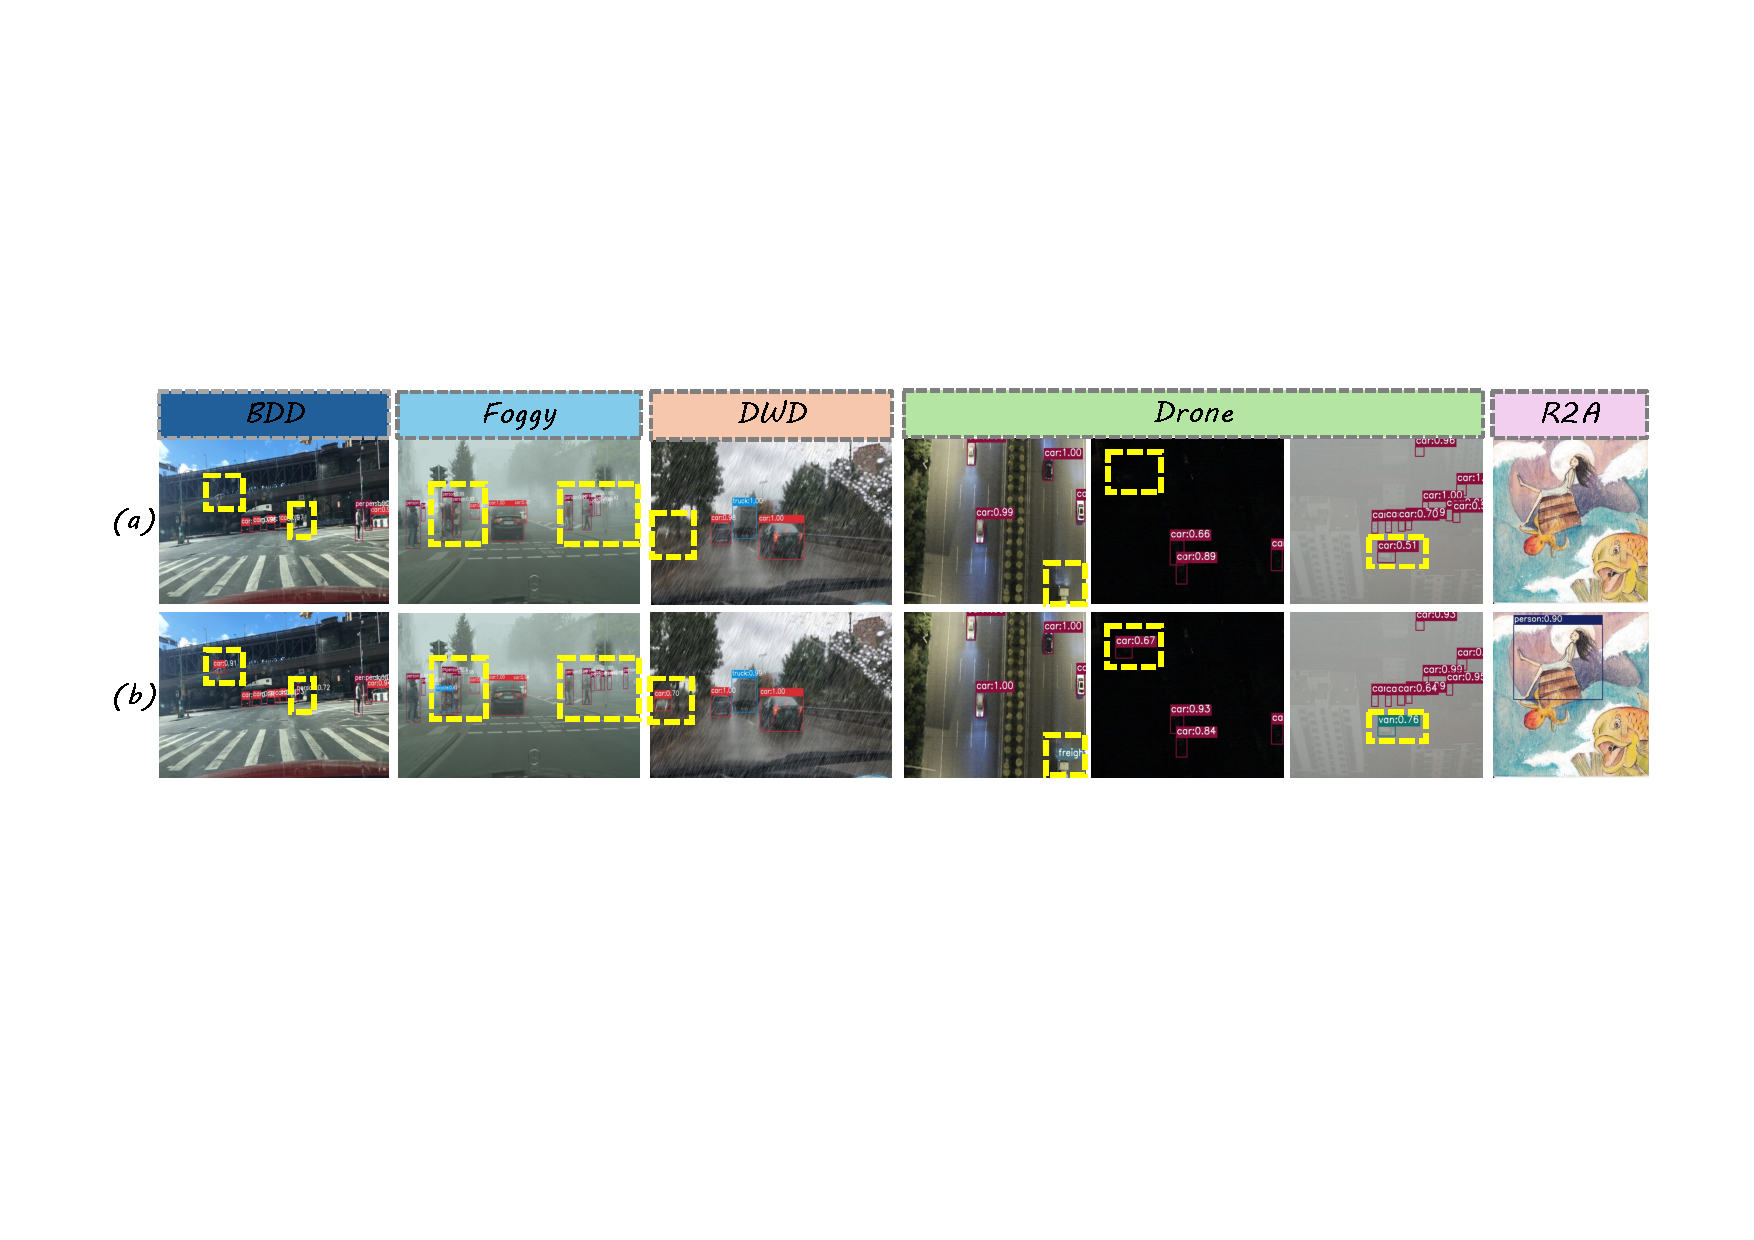
\includegraphics[width=1.02\textwidth]{figs/visualization.pdf}
    \caption{Visualization results on four domain adaptation benchmarks: BDD100K (BDD)~\cite{yu2020bdd100k}, FoggyCityscapes (Foggy)~\cite{sakaridis2018semantic}, Diverse Weather Datasets (DWD)~\cite{wu2022single}, Diverse Weather DroneVehicle, and Real-to-Artistic (R2A)~\cite{inoue2018cross}. (a) shows the baseline model with the DINOv3 backbone, while (b) presents the results of our proposed \textbf{\textit{Bridge}} method. Best viewed with zooming in.}
    \label{fig:visualization}
    \vspace{-6pt}
\end{figure*}

\vspace{4pt}
\noindent\textbf{Qualitative results.} 
Figure~\ref{fig:visualization} presents qualitative visualizations using DINOv3 as the backbone detector. \textbf{\textit{Bridge}} produces more robust and precise detections under various challenging scenarios, showing fewer false alarms and missed objects compared to the baseline.

\subsection{Ablation Study}
\noindent{\textbf{Effect of Causal Basis Block}:}
Table~\ref{tab:cbb_componet} reports the ablation results of different components within our CBB module. We adopt DINOv3, SAM, and SD as the backbone networks, train them on Cityscapes, and evaluate on Foggy Cityscapes. Compared to the baseline, incorporating Low-Rank Basis  (LRB) leads to mAP improvements of $3.2$, $3.4$, and $1.3$ for DINOv3, SAM, and SD, respectively. Further adding \textit{Sample Queries} for aggregating information from multiple samples provides additional gains of $0.7$, $0.7$, and $0.5$ mAP. These results demonstrate the effectiveness of the low-rank basis and \textit{Sample Queries} components in the proposed CBB module.

We further re-implement the front-door adjustment proposed in GOAT~\cite{wang2024vision} using a cross-attention mechanism~\cite{vaswani2017attention}, which is inserted between multi-scale feature layers (implementation details are provided in the supplementary material). As shown in Table~\ref{tab:facl}, this variant, denoted as FACL, yields only limited improvements across datasets. In contrast, our CBB consistently achieves higher mAP on all benchmarks, highlighting the superior effectiveness of our causal modeling design.

\vspace{4pt}
\noindent{\textbf{Effect of Basis numbers}:}
Table~\ref{tab:basis_ratio} presents the results of varying the number of bases used in our CBB module. 
We adopt DINOv3, SAM, and SD as the backbone networks, train them on Cityscapes, and evaluate on Foggy Cityscapes.
As discussed in Section~\ref{sec:coefficients_estimation}, the basis matrix is defined as $\mathcal{B} = [b_1, \dots, b_K] \in \mathbb{R}^{K \times C}$ with $K < C$, where a smaller $K$ filters out more redundant information and retains more general representations. In this experiment, we investigate how different VFMs respond to varying basis ratios, where the ratio denotes the proportion of $K$ relative to $C$.

We observe that for the strong backbone DINOv3, using only $12.5\%$ of the original feature dimension yields the best performance, suggesting that a compact basis space effectively captures the essential representations. In contrast, SAM and SD achieve optimal results at higher ratios (around $50\%$–$70\%$), indicating that models with weaker representation capacity need a larger basis set to preserve sufficient feature diversity.

\vspace{4pt}
\noindent{\textbf{Generalization across Detectors}:}
Table~\ref{tab:ab_detectors} presents the generalization results of \textbf{\textit{Bridge}} across different object detectors.
In addition to the anchor-based Faster R-CNN, we further evaluate two representative anchor-free detectors, Sparse R-CNN~\cite{sun2021sparse} and TOOD~\cite{feng2021tood}.
Consistent improvements are observed when integrating \textbf{\textit{Bridge}} into both frameworks, highlighting the strong generalization ability of \textbf{\textit{Bridge}} across diverse detection frameworks.

    
    % \vspace{-3mm}
    
    \begin{table}[htbp]
        \centering
        \caption{Effect of Low-Rank Basis and Sample Queries within CBB.}
        \vspace{-4pt}
        \label{tab:component}
        \footnotesize
        \renewcommand{\arraystretch}{1}
    \setlength{\tabcolsep}{4pt}  % 
    
    \resizebox{\columnwidth}{!}{%
        \begin{tabularx}{\linewidth}{%
        >{\centering\arraybackslash}X % Backbone
        |>{\centering\arraybackslash}p{2.cm} % LRR
        |>{\centering\arraybackslash}p{2.3cm} % Sample Queries 
        |>{\centering\arraybackslash}X % mAP
        }
        \toprule
        \textbf{Backbone} & \textbf{LRB} & \textbf{Sample Queries} & \textbf{mAP} \\
        \midrule
        \multirow{3}{*}{DINOv3}  &           &   &  57.7        \\
                                 & \ding{51} &  & 60.9          \\
                                 & \ding{51} & \ding{51} & \textbf{61.6} \\
        \midrule
        \multirow{3}{*}{SD}      &           &  & 51.8           \\
                                 & \ding{51} &  & 53.1          \\
                                 & \ding{51} & \ding{51} & \textbf{53.6} \\
        \midrule
        \multirow{3}{*}{SAM}    &           &     & 45.8         \\
                                & \ding{51} &  & 49.2           \\
                                 & \ding{51} & \ding{51} & \textbf{49.9} \\
        \bottomrule
        \end{tabularx}
        }
        \label{tab:cbb_componet}
        \vspace{-6pt}
        \end{table}

\begin{table}[htbp]
\centering
\caption{DG Results (\%) on five benchmark.}
\vspace{-4pt}
\label{tab:map_five_datasets}
\footnotesize
\begin{tabularx}{\linewidth}{
>{\raggedright\arraybackslash}X |
>{\centering\arraybackslash}p{0.8cm} |
>{\centering\arraybackslash}p{0.8cm} |
>{\centering\arraybackslash}p{0.8cm} |
>{\centering\arraybackslash}p{0.8cm} |
>{\centering\arraybackslash}p{0.8cm}
}
\toprule
\textbf{Method} & \textbf{BDD} & \textbf{Foggy} & \textbf{DWD} & \textbf{Drone} & \textbf{R2A} \\
\midrule
Baseline & 57.8 & 57.7 & 48.6 & 47.1 & 72.7 \\
FACL~\cite{wang2024vision}     & 58.5 & 60.5 & 48.2 &  46.8 & 71.6 \\
Ours      & \textbf{58.9} & \textbf{61.6} & \textbf{50.8} & \textbf{48.4} & \textbf{73.3} \\
\bottomrule

\end{tabularx}
\label{tab:facl}
\end{table}

\begin{table}[htbp]
    \centering
    \caption{Ablation Study on Basis Ratio}
    \vspace{-4pt}
    \label{tab:basis_ratio}
    \footnotesize
    \renewcommand{\arraystretch}{1}
    \setlength{\tabcolsep}{6pt}  
    \resizebox{\columnwidth}{!}{%
    \begin{tabularx}{\linewidth}{>{\raggedright\arraybackslash}m{0.15\linewidth}|>{\centering\arraybackslash}X>{\centering\arraybackslash}X>{\centering\arraybackslash}X>{\centering\arraybackslash}X>{\centering\arraybackslash}X}
    \toprule
    \multirow{2}{*}{\textbf{Backbone}} & \multicolumn{5}{c}{\textbf{Basis Ratio}} \\
    \cmidrule(lr){2-6}
     & 90\% & 70\% & 50\% & 25\% & 12.5\% \\
    \midrule
    DINOv3 & 60.9 & 61.1 & 61.3 & 61.3 & \textbf{61.6} \\
    SAM    & 48.5 & 48.7 & \textbf{49.9} & 48.5 & 48.4 \\
    SD     & 52.8 & \textbf{53.6} & 52.5 & 52.5 & 51.9 \\
    \bottomrule
    \end{tabularx}
    }
    \vspace{-6pt}
\end{table}
\begin{table}[htbp]
\centering
\caption{Generalization comparison across different detectors on five datasets.  Best values are in \textbf{boldface}.}
\vspace{-4pt}
\label{tab:generalization_detectors}
\footnotesize
\begin{tabularx}{\linewidth}{
>{\raggedright\arraybackslash}X |
>{\centering\arraybackslash}p{0.6cm} |
>{\centering\arraybackslash}p{0.6cm} |
>{\centering\arraybackslash}p{0.6cm} |
>{\centering\arraybackslash}p{0.6cm} |
>{\centering\arraybackslash}p{0.6cm}
}
\toprule
\textbf{Detector} & \textbf{BDD} & \textbf{Foggy} & \textbf{DWD} & \textbf{Drone} & \textbf{R2A} \\
\midrule
Sparse R-CNN~\cite{sun2021sparse} &36.3  &43.2  &42.3  &28.7  &60.9  \\
 \rowcolor{lightgreen}
\textit{\textbf{Ours}}     & \textbf{37.6} & \textbf{44.6} &\textbf{45.6}  &\textbf{30.3}  &\textbf{62.1}  \\
\midrule
TOOD~\cite{feng2021tood}         & 56.1 & 56.6  & 47.3 & 46.8 &70.3  \\
 \rowcolor{lightgreen}
\textit{\textbf{Ours}}    & \textbf{59.4} & \textbf{60.8} &\textbf{50.1}  & \textbf{50.3} &\textbf{72.8}  \\
\bottomrule
\end{tabularx}
\label{tab:ab_detectors}
% \vspace{-6pt}
\end{table}


\vspace{4pt}
\noindent{\textbf{Limitation}:}
In this work, we propose CBB to approximate expectations for formulating the front-door adjustment (Equation~\ref{equ:front_door_adjustment}). However, the complexity of the representation space makes obtaining closed-form solutions intractable~\cite{wang2024vision,yang2021deconfounded}. Consequently, CBB approximates these expectations using the low-rank bases and sample queries, rather than deriving analytical solutions. 